\chapter{The Stock Management Web Application} % Materials \& Methods
\label{chap:app}
\textbf{In this section I will represent what you did in the internship. The project as well as its Conception and design, the Tools Used and its Realisation.}

%\Blindtext
\section{Introduction}%Summary
	During the last two weeks of the internship, I was given the task to design and implement A stock management Web application for Tunisie Telecom's Stock of Fiber Optics, all for the benefits of a DBMS:  Efficiency, Reliability, Convenience, Safety, Multi-User storage of and access to massive amounts of persistent data.
\section{Tools Used}
	During my internship I used a number of tools including: \\
		- Kali Linux 2019.3 \& Elementary OS 5.0 Juno\\
		- LAMP 7.3.9 \\
		- Git 2.23.0 \& GitHub\\
		- Sublime Text 3.0 \\
		- MikTex 2.9.7100 \& TexWorks 0.6.3 \\
\section{Analysis \& Conception} % Database UML & class diagram & Use case
	In this Section I will Present a detailed analysis of the problem at hand and its proposed Conception.
\subsection{Analysis}
	
	\begin{figure}[ht!] % supposedly places it here ...
  \centering
  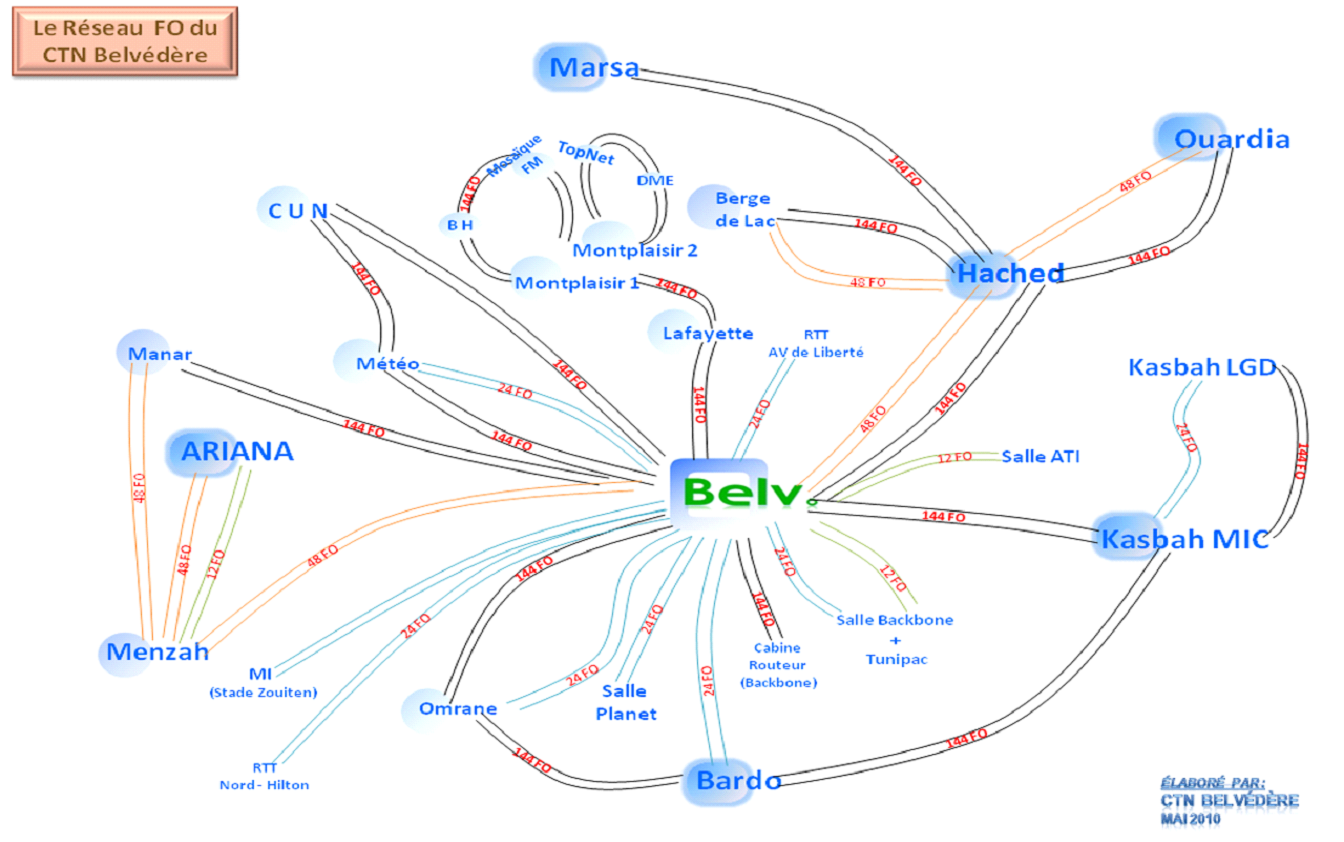
\includegraphics[width=\linewidth]{DTC_Belvedere}
  \caption[DTC Belvedere]{Optic Fibers Map}%\index{Goku il-king}}%
  \label{fig:OFMap}
\end{figure}


\subsection{Conception}
\begin{figure}[ht!] % supposedly places it here ...
  \centering
  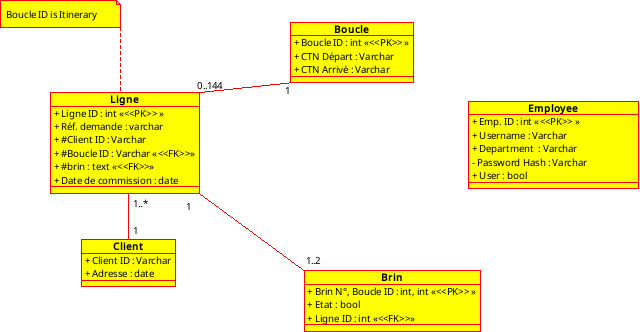
\includegraphics[width=\linewidth]{Class_Diagram}
  \caption[Class Diagram]{Conception}%\index{Goku il-king}}%
  \label{fig:DiagClass1}
\end{figure}

\section{Realisation}%Summary

\blindtext
\begin{figure}[ht!] % supposedly places it here ...
  \centering
  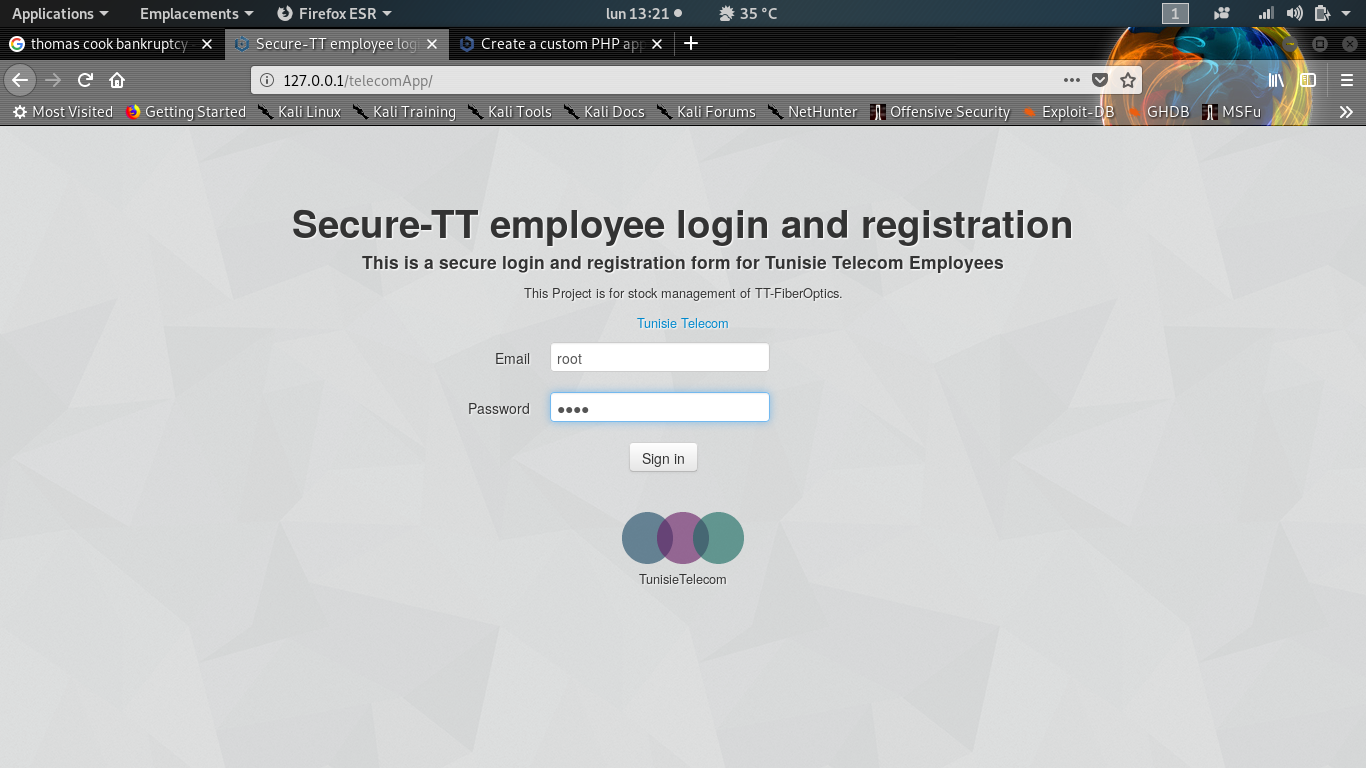
\includegraphics[width=\linewidth]{Login}
  \caption[Login]{Conception}%\index{Goku il-king}}%
  \label{fig:Login}
\end{figure}

\begin{figure}[ht!] % supposedly places it here ...
  \centering
  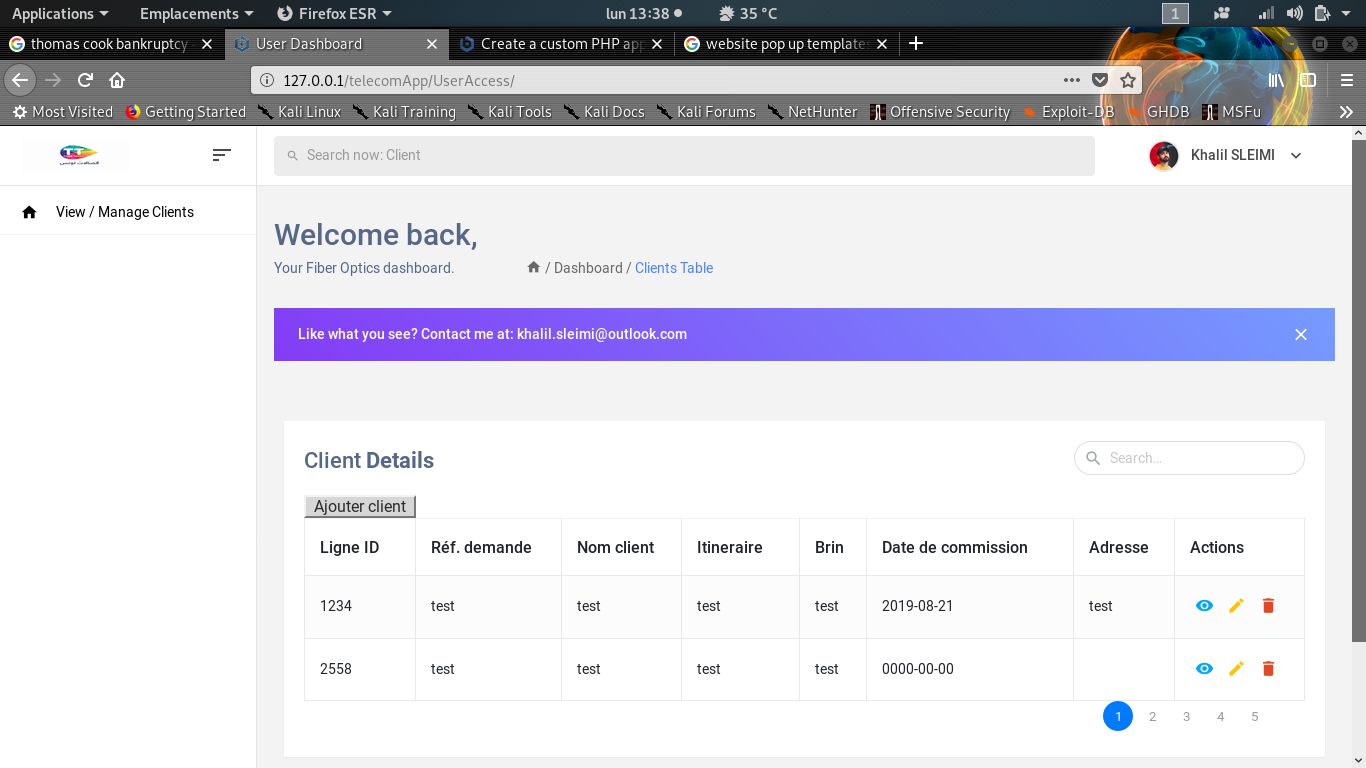
\includegraphics[width=\linewidth]{UserTableau}
  \caption[UserClientsTable]{Conception}%\index{Goku il-king}}%
  \label{fig:UserTable}
\end{figure}

\begin{figure}[ht!] % supposedly places it here ...
  \centering
  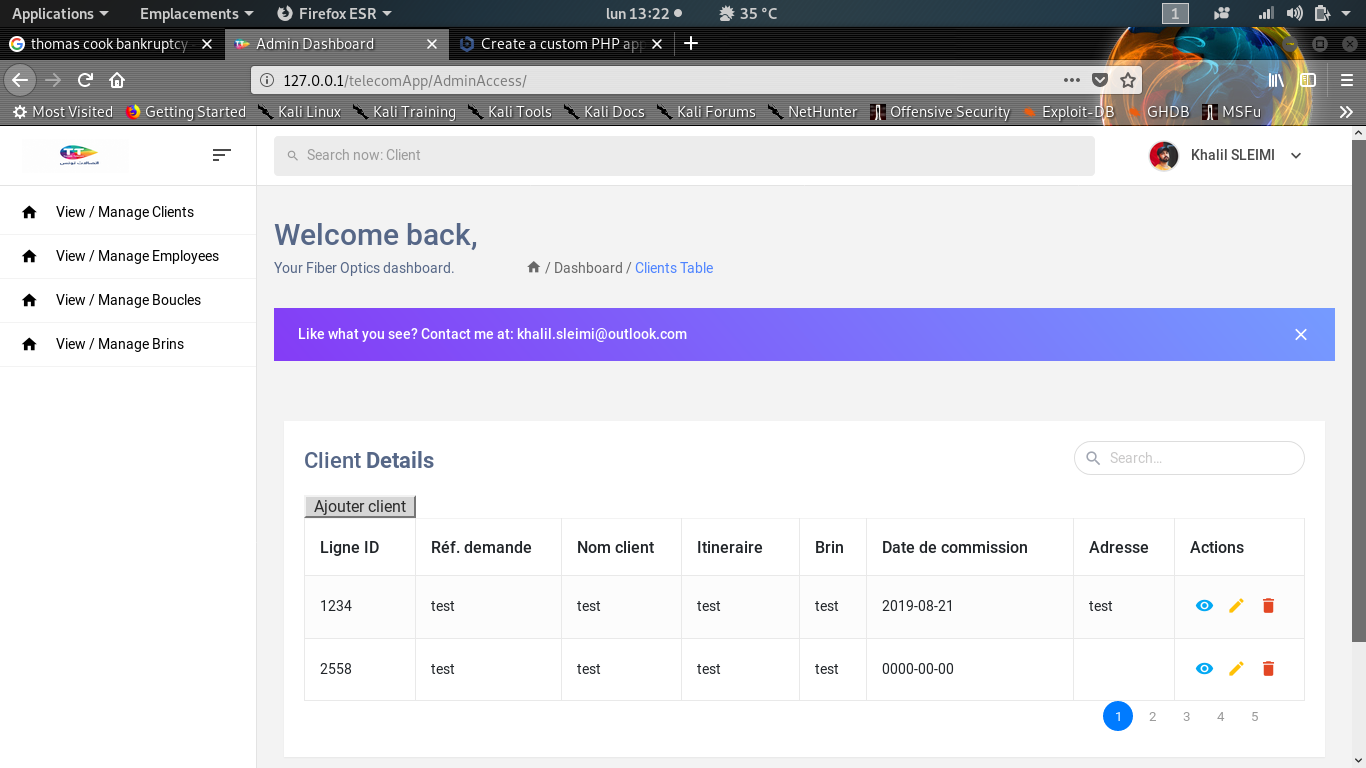
\includegraphics[width=\linewidth]{AdminTableau}
  \caption[AdminClientsTable]{Conception}%\index{Goku il-king}}%
  \label{fig:AdminClientsTable}
\end{figure}

\begin{figure}[ht!] % supposedly places it here ...
  \centering
  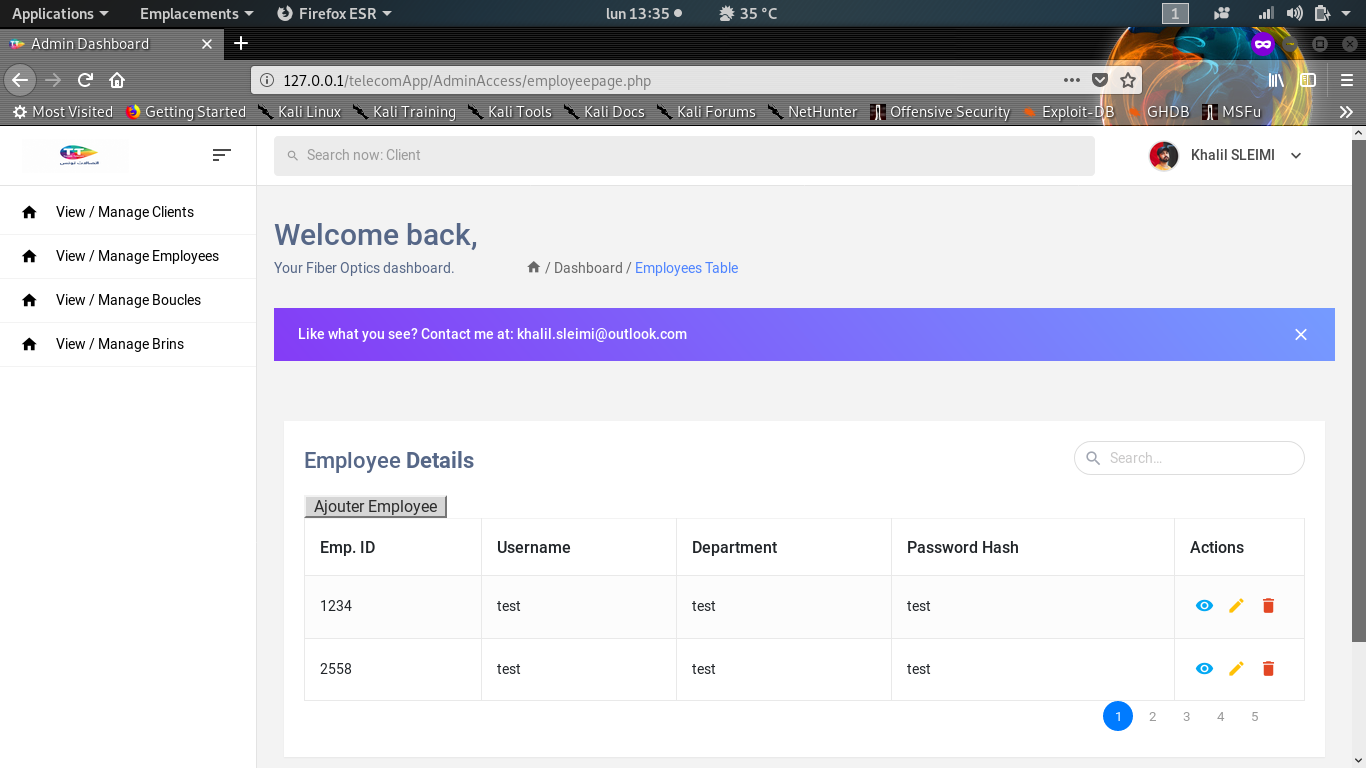
\includegraphics[width=\linewidth]{AdminEmployeeTableau}
  \caption[AdminEmployeeTable]{Conception}%\index{Goku il-king}}%
  \label{fig:AdminEmployeeTable}
\end{figure}

\begin{figure}[ht!] % supposedly places it here ...
  \centering
  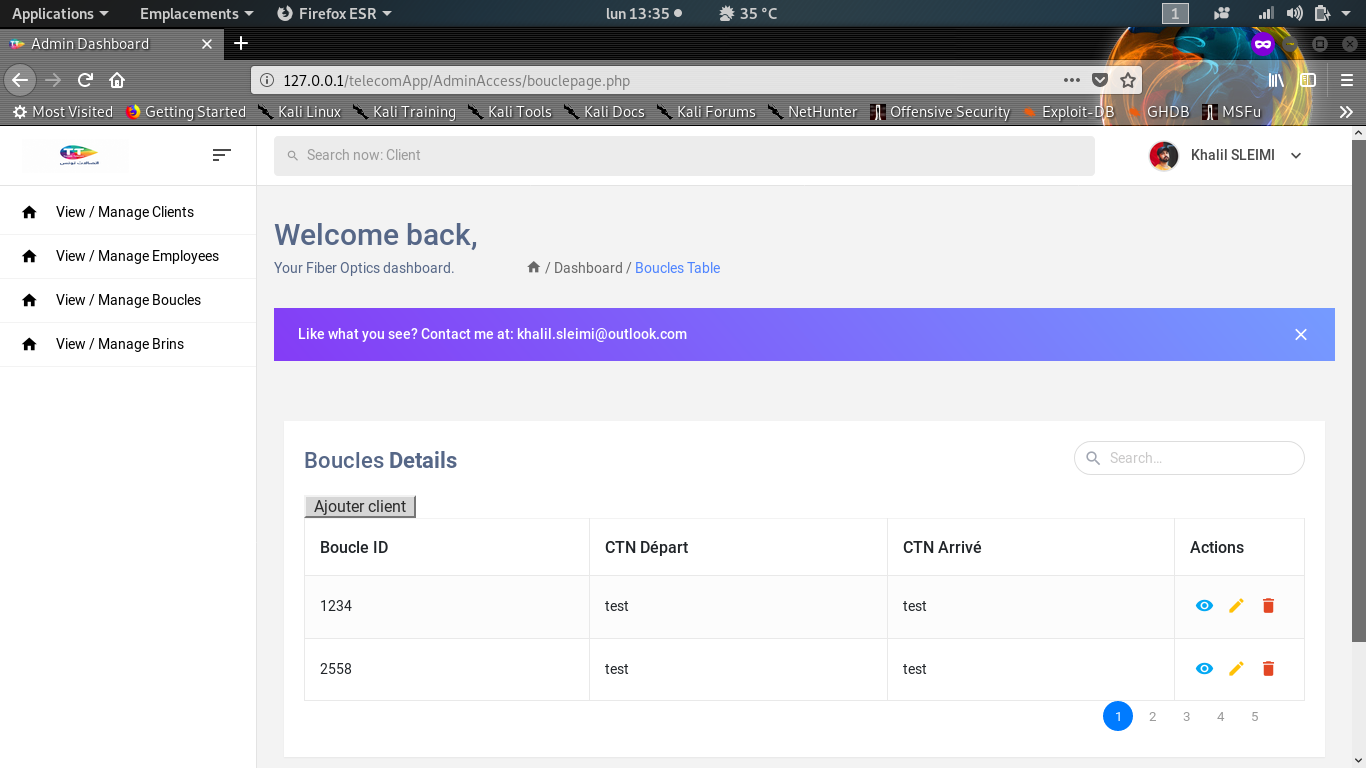
\includegraphics[width=\linewidth]{AdminBouclesTableau}
  \caption[AdminBouclesTable]{Conception}%\index{Goku il-king}}%
  \label{fig:AdminBouclesTable}
\end{figure}

